\documentclass[10pt]{article}
\usepackage{tocloft}
\usepackage[utf8]{inputenc}
% \usepackage{hyperref}
\usepackage{geometry}

% Page Dimensions
\geometry{
  a4paper,
  total={170mm,257mm},
  left=10mm,
  top=14mm,
  right=10mm,
  bottom=12mm
}

\usepackage{graphicx}
\usepackage{titling}
\usepackage{fancyhdr}
\usepackage{titlesec}
\usepackage{wrapfig}
\usepackage{graphicx}
\usepackage{comment}
\usepackage[title,toc,titletoc,page]{appendix}
\usepackage{bold-extra}
\usepackage[scaled=0.85]{beramono}
\usepackage{enumitem}
\usepackage{multicol}
\usepackage{array}
\usepackage{mathtools,amssymb}
\usepackage[hidelinks]{hyperref}
\usepackage{titlesec}

% Adjust the size of the "Appendices" section title
\titleformat{\section}[block]{\normalfont\small\bfseries}{\thesection}{1em}{}



%  Bibliography
\usepackage{biblatex}
% Section formatting
\titleformat{\section}
  {\normalfont\large\bfseries}
  {\thesection}
  {.5em}
  {}

% Subsection formatting
\titleformat{\subsection}
  {\normalfont\large\bfseries}
  {\thesubsection}
  {1em}
  {}

% Subsubsection formatting
\titleformat{\subsubsection}
  {\normalfont\normalsize\bfseries}
  {\thesubsubsection}
  {1em}
  {}

% Section spacing
\titlespacing*{\section}
  {0pt} % Left margin
  {0.5ex plus .1ex minus .1ex} % Space before section
  {0.25ex plus .1ex minus .1ex} % Space after section

% Subsection spacing
\titlespacing*{\subsection}
  {0pt} % Left margin
  {0.5ex plus .1ex minus .1ex} % Space before subsection
  {0.25ex plus .1ex minus .1ex} % Space after subsection

% Subsubsection spacing
\titlespacing*{\subsubsection}
  {0pt} % Left margin
  {0.5ex plus .1ex minus .1ex} % Space before subsubsection
  {0.25ex plus .1ex minus .1ex} % Space after subsubsection

\title{Study of Garbage Collection in Lua}
\author{Bratin Mondal}

\fancypagestyle{plain}{
    \fancyhf{}
    \fancyhead[L]{Garbage Collection in Lua}
    \fancyhead[R]{Bratin Mondal}
}

\makeatletter
\def\@maketitle{%
  \newpage
  \null
  \begin{center}%
    {\LARGE \@title \par}%
  \end{center}%
  \par
  }
\makeatother

\usepackage{lipsum}  % Remove or replace with actual content
\usepackage{cmbright}

% No spacing between items in itemize
\usepackage{enumitem}
\setlist{nosep} % Removes extra space in lists

%  Reduce the font size of the document
\renewcommand{\normalsize}{\small}
\setlist[enumerate,1]{itemsep=0pt, parsep=0pt, topsep=0pt, partopsep=0pt}

\begin{document}

\maketitle

\noindent

\begin{flushleft}
    \textbf{Name:} Bratin Mondal \hfill \textbf{Course Code:} CS60203 \\
    \textbf{Roll Number:} 21CS10016 \hfill \textbf{Course Name:} Design Optimization of Computing Systems
\end{flushleft}


\section{Introduction}
Lua, a dynamically typed language, originally used a basic mark-and-sweep garbage collector. Lua 5.1 introduced an incremental collector to improve performance by interleaving collection with program execution. Although Lua 5.2's generational collector aimed to optimize memory management, it was reverted in 5.3 due to challenges. The generational collector was reintroduced with enhancements in Lua 5.4. This report examines the evolution and implementation of Lua's garbage collection mechanisms.


\section{Fundamentals of Lua's Garbage Collection}

To understand Lua's garbage collectors, we must first grasp the basics of its memory management. Lua, written in C, manages memory through objects of eight basic types: \texttt{nil}, \texttt{boolean}, \texttt{number}, \texttt{string}, \texttt{function}, \texttt{userdata}, \texttt{thread}, and \texttt{table}. These objects are typically organized into type-specific lists for memory management.




% TODO: FINALIZED
\subsection{Root Set} \label{sec:root_set}

In Lua's garbage collection mechanism, only objects that are accessible from the root set are preserved during a garbage collection cycle. The root set comprises objects that are directly reachable and thus considered live. In Lua, the root set includes:

\begin{itemize}
    \item The registry, which holds the global table (\_G), the main thread, and the \texttt{package.loaded} table that tracks loaded modules.
    \item Shared metatables, which are used across various parts of the Lua environment.
\end{itemize}

\subsection{Tri-Color Marking} \label{sec:tri_color_marking}

\begin{wrapfigure}{r}{0.15\textwidth}
  \centering
  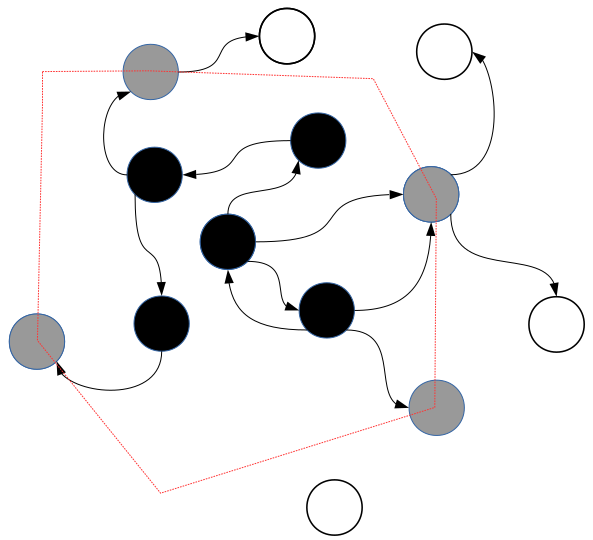
\includegraphics[width=0.15\textwidth]{WGB.png}
  \caption{Tri-Color Marking}
  \label{fig:tri-color-marking}
\end{wrapfigure}

Lua's garbage collector marks objects with three colors: white, gray, and black.

\begin{itemize}
  \item \textbf{White}: Objects not reachable from the root set.
  \item \textbf{Gray}: Objects reachable from the root set but with unmarked references.
  \item \textbf{Black}: Objects reachable from the root set with all references marked.
\end{itemize}

Lua uses two types of white objects, \texttt{WHITE0} and \texttt{WHITE1}, to differentiate between objects marked in the current and previous cycles. The main invariant is that no black object can reference a white object, with gray objects forming the boundary between them. Gray objects must be revisited before the cycle ends and kept in the \texttt{gray} list. Objects demoted from black to gray are added to the \texttt{grayagain} list for revisiting during the atomic [\ref{sec:gcsatomic}] phase.

\subsection{Age-Based Marking} \label{sec:age_based_marking}



In Lua's generational garbage collector, objects are assigned an age along with their color, which is updated after each cycle. The age categories are:

\textbf{G\_NEW} denotes objects created in the current cycle. \textbf{G\_SURVIVAL} indicates objects that have survived at least one cycle. \textbf{G\_OLD0} marks objects classified as old in this cycle. \textbf{G\_OLD1} represents objects that having completed first full cycle as old. \textbf{G\_OLD} describes objects that have survived at least two full cycles as old. \textbf{G\_TOUCHED1} refers to old objects with references to new objects in the current cycle, while \textbf{G\_TOUCHED2} applies to old objects with references to new objects from the previous cycle. A key invariant is that truly old objects cannot reference new ones.
\
\subsection{Work and Debt} \label{sec:debt_and_work}

In incremental and generational garbage collectors, work is divided into manageable steps, measured by metrics such as bytes scanned, objects marked, or finalizers invoked (e.g., scanning 1 byte is 1 unit of work, invoking a finalizer is 50 units). 

Debt, representing the remaining work, adjusts with object allocation and collection. It increases with allocation and decreases with collection, and the system triggers the next cycle when debt reaches a threshold. This mechanism maintains efficient workload management and balance in the garbage collection process. Details on debt management for specific collectors will follow.



\subsection{Freeing an Object} \label{sec:freeing_object}

\textbf{freeobj} handles the deallocation of unreachable objects. \textbf{luaH\_free} deallocates Lua tables by freeing the hash part with \textbf{freehash}, the array part with \textbf{luaM\_freearray}, and the table structure with \textbf{luaM\_free}. 

\textbf{luaM\_free} is a macro that calls \textbf{luaM\_free\_}, which performs the actual memory deallocation via \textbf{l\_alloc} using standard C library functions.


\section{Stages of a Garbage Collection Cycle} \label{sec:gc_cycle}

Understanding the stages of a garbage collection cycle is essential before exploring the different garbage collectors in Lua. Although some stages are common to all collectors, others differ based on the specific type of collector.

The Lua garbage collection cycle involves nine stages: \textbf{GCSpropagate}, \textbf{GCSenteratomic}, \textbf{GCSatomic}, \textbf{GCSswpallgc}, \textbf{GCSswpfinobj}, \textbf{GCSswptobefnz}, \textbf{GCSswpend}, \textbf{GCScallfin}, and \textbf{GCSpause}. The cycle starts and ends in the \textbf{GCSpause} state, with the \textbf{singlestep} function managing the execution of each stage and transitioning between states. Details of each stage's tasks are outlined below.


\subsection{GCSpause} \label{sec:gcspause}

The collection process begins in the \textbf{GCSpause} state, where the \textbf{restartcollection} function is invoked. This function clears the gray list and marks the root set, global metatables, and registry. It also marks any objects that were being finalized in the previous cycle but whose finalizers have not yet been executed. After completing these tasks, the state transitions to \textbf{GCSpropagate}.


\subsection{GCSpropagate} \label{sec:gcspropagate}

In the \textbf{GCSpropagate} state, the \texttt{gray} list is traversed until empty. The \textbf{propagatemark} function is responsible for marking various object types. Objects that require further processing in the atomic phase are added to the \texttt{grayagain} list. When no more gray objects remain, the state transitions to \textbf{GCSenteratomic}.


\subsection{GCSenteratomic} \label{sec:gcsenteratomic}

The \textbf{GCSenteratomic} function calls the \textbf{atomic} function, which changes the state to \textbf{GCSatomic}. This is the entry point for the atomic phase through the \textbf{singlestep} function.


\subsection{GCSatomic} \label{sec:gcsatomic}

The \textbf{GCSatomic} phase is crucial in the garbage collection cycle, especially for incremental and generational collectors, and must complete in a single pause. It involves several key steps:

First, the current \texttt{grayagain} list [\ref{sec:tri_color_marking}] is saved in a temporary variable, and \texttt{grayagain} is set to \texttt{NULL}. The running thread, global metatables, and registry are then marked. Next, the \texttt{gray} [\ref{sec:tri_color_marking}] and \texttt{grayagain} lists are traversed to mark all reachable objects.

The \textbf{convergeephemerons} function is called to process \texttt{ephemeron tables} [\ref{sec:weak_tables}], propagating marks from keys to values until no more marks can be propagated, with alternating traversal directions to improve efficiency. \texttt{Weak tables} [\ref{sec:weak_tables}] are then updated to clear values with dead keys, and the status of these tables is recorded.

Objects with finalizers marked for collection are moved to the \texttt{tobefnz} list and re-marked due to potential resurrection [\ref{sec:resurrection}]. The \textbf{propagateall} function is invoked to propagate changes from re-marking, followed by another call to \textbf{convergeephemerons} for additional propagation in ephemeron tables.

Finally, the API string cache is cleared, and the current white is switched to the other white (from \texttt{WHITE0} to \texttt{WHITE1} or vice versa) to distinguish between objects marked in this step and those in the subsequent marking step.

At the end of this phase, the \textbf{entersweep} function is called, changing the state to \textbf{GCSswpallgc}. This function updates the object list pointer to refer to an object within the list (bypassing the header), skips dead objects using \textbf{sweeptolive}, and estimates the total memory allocated.

Notably, this is the only phase where the invariant of no black object referencing a white object [\ref{sec:tri_color_marking}] is violated.



\subsection*{sweepstep Function} \label{sec:sweepstep}

The \textbf{sweepstep} function is vital in the garbage collection process. It utilizes the \textbf{sweeplist} function to process a list of objects. During this phase:

First, each object is checked; if its color is non-current \texttt{white} (indicating it is dead), it is freed using the \textbf{freeobj} [\ref{sec:freeing_object}] function. Objects that are not dead have their color updated to current white, preparing them for the next cycle. The function removes up to \texttt{GCSWEEPMAX} objects from the list and returns a pointer to the next object for future processing. Additionally, the total memory allocated is adjusted by subtracting the size of the freed objects.


Following this, the \textbf{sweepstep} function updates the object list pointer to the next list to be processed. If the object list pointer is NULL, the state is changed to \textbf{GCSswpend}.

\subsection{GCSswpallgc State}
In the \textbf{GCSswpallgc} state, the \textbf{sweepstep} function [\ref{sec:sweepstep}] is called to sweep all regular objects. This process involves sweeping the list of all regular objects, updating their colors, and freeing dead objects. Once the list is fully processed, the state transitions to \textbf{GCSswpfinobj}.

\subsection{GCSswpfinobj State}
During the \textbf{GCSswpfinobj} state, the \textbf{sweepstep} function [\ref{sec:sweepstep}] processes the list of all objects with finalizers. When the end of this list is reached, the state transitions to \textbf{GCSswptobefnz}.

\subsection{GCSswptobefnz State}
In the \textbf{GCSswptobefnz} state, the \textbf{sweepstep} function [\ref{sec:sweepstep}] sweeps the list of objects marked for finalization (Objects with finalizer marked as dead). Once this list is fully processed, the state transitions to \textbf{GCSswpend}.

\subsection{GCSswpend State}
When in the \texttt{GCSswpend} state, the \textbf{checkSizes} function is invoked to assess the sizes of the string table and attempt to shrink it if possible. Subsequently, the state transitions to \textbf{GCScallfin}.

\subsection{GCScallfin State}
In the \textbf{GCScallfin} state, the \textbf{runafewfinalizers} function executes a limited number of finalizers (up to 10). This approach prevents excessive delays that could result from running all finalizers in one step. Once this process is completed, the state changes to \textbf{GCSpause} marking the end of the garbage collection cycle.

\section{Stop-the-World Garbage Collection} \label{sec:stop_the_world}
In Lua, a stop-the-world garbage collection cycle can be initiated by calling the \textbf{luaC\_fullgc} function. From the user space, this can be triggered by first turning off the default incremental mode using \textbf{lua\_gc(L, LUA\_GCSTOP, 0)}(\texttt{lapi.c}) which sets \texttt{gcstp} to \texttt{GCSTPUSR} and then calling \textbf{lua\_gc(L, LUA\_GCRESTART, 0)}(\texttt{lapi.c}) which clears any remaining cycles and sets \texttt{gcstp} to 0 and sets \texttt{GCdebt} to 0 by calling \textbf{luaE\_setdebt}(\texttt{lstate.c}) function.
 Finally, the \textbf{lua\_gc(L, LUA\_GCCOLLECT, 0)}(\texttt{lapi.c}) function call will start the garbage collection cycle.

The \textbf{luaC\_fullgc} function executes all the stages of a garbage collection cycle in a single pause by invoking the \textbf{fullinc} function.
The flow of the function calls are as follows as found in the graph (some functions from source code are not visible possibly due to function inlining or less instructions spent)
%  reduce vertical space
\vspace{-1em}

\[
\textbf{lua\_gc(L, LUA\_GCCOLLECT, 0)} \rightarrow \textbf{luaC\_fullgc} \rightarrow \textbf{singlestep} \rightarrow \textbf{entersweep} \rightarrow \textbf{sweeplist} \rightarrow \textbf{freeobj} \rightarrow \textbf{luaH\_free} \rightarrow \textbf{luaM\_free} \rightarrow \textbf{l\_alloc}
\]

\subsection{Execution Flow}

\begin{enumerate}
    \item \textbf{lua\_gc(L, LUA\_GCCOLLECT, 0)} triggers the garbage collection cycle.
    
    \item \textbf{luaC\_fullgc} executes all stages of the garbage collection cycle in a single pause. It calls the \textbf{fullinc} function to manage incremental steps and uses the \textbf{luaC\_runtilstate} function to transition between states with the \textbf{singlestep} [\ref{sec:gc_cycle}] function.
  
    \item \textbf{singlestep} completes any remaining steps from the previous cycle before starting a new one. If any marked objects are found, they are processed in the \textbf{entersweep} function to mark them back to white, and the state is reset to \textbf{GCSpause}.
  
    \item The \textbf{Marking Phase} begins. In the \textbf{GCSpause} state, the root set, global metatables, and registry are marked. The \textbf{GCSpropagate} state is skipped as traversal will eventually be completed in the \textbf{GCSatomic} state.
  
    \item \textbf{singlestep} advances the garbage collection cycle step-by-step, transitioning between states. In the atomic phase, the gray list is traversed, and objects are marked as black. The \textbf{convergeephemerons} function processes ephemeron tables, and weak tables are updated to clear dead keys.

    \item The \textbf{Sweeping Phase} begins with the \textbf{GCSswpallgc} state, followed by \textbf{GCSswpfinobj} and \textbf{GCSswptobefnz}. The \textbf{sweepstep} function [\ref{sec:sweepstep}] is called to sweep through lists of objects, freeing dead objects and updating memory allocation.  Object traversal follows the steps in the \textbf{sweepstep} function, first for regular objects and then for objects with finalizers.

    \item The \textbf{freeobj} [\ref{sec:freeing_object}] function deallocates memory using \textbf{luaH\_free} for tables and \textbf{luaM\_free} for other objects. The \textbf{luaM\_free} function uses \textbf{l\_alloc} to deallocate memory with standard C library functions.
  \end{enumerate}

  Essentially, the stop-the-world garbage collection cycle in Lua complets all stages in a single pause, ensuring that all objects are marked, swept, and finalized before the cycle ends as discussed in section [\ref{sec:gc_cycle}]. 
  
  During a stop-the-world garbage collection cycle, the entire program is paused until the collection completes. This pause can be noticeable in programs with large heaps or heavy load, leading to potential interruptions in responsiveness, which is problematic for real-time applications requiring low latency.



\section{Incremental Garbage Collection} \label{sec:incremental_gc}
In Lua, the incremental garbage collector is designed to minimize the impact of garbage collection pauses on program execution. Instead of performing the entire garbage collection cycle in one go, the incremental collector interleaves the collection process with program execution. This approach allows the garbage collector to perform small, incremental steps reducing the duration of each pause.
\subsection{Parameters}
Three parameters control the behavior of the incremental garbage collector:
\subsubsection{Pause} \label{sec:pause}
The garbage collector's pause setting controls the delay before starting a new cycle. The collector begins a new cycle when memory usage reaches \texttt{n\%} of the usage after the last collection. Larger values result in a less aggressive collector. A value of 200 means the collector waits for memory usage to double before initiating a new cycle. The default value is 200, with a maximum of 1000.
\subsubsection{Step multiplier} \label{sec:step_multiplier}
The garbage-collector step multiplier controls the speed of the collector relative to memory allocation by determining how many elements are marked or swept for each kilobyte of memory allocated. Larger values make the collector more aggressive, increasing the size of each incremental step. It is recommended to avoid values below 100, as they may cause the collector to become too slow and potentially prevent it from completing a cycle. The default value is 100, and the maximum allowable value is 1000. Essntailly, it converts debt [\ref{sec:debt_and_work}] from bytes to work units as
\begin{equation}
  \text{debt} = \frac{g \rightarrow \text{GCdebt}}{\text{WORK2MEM}}\times{\text{stepmul}}
\end{equation}
Where \text{WORK2MEM} is a macro that converts gives size of Tagged Value (Basic representation of values in Lua: an actual value plus a tag with its type.)
\subsubsection{Step size} \label{sec:step_size}
The garbage-collector step size controls the amount of memory allocated by the interpreter before performing a garbage collection step.
This parameter is logarithmic: a value of \( n \) means the interpreter will allocate \( 2^n \) bytes between two consecutive steps of a single cycle. Large value, such as 60, turns the collector into a stop-the-world (non-incremental) collector. The default value is 13, which results in steps of approximately 8 KB. 

\subsection{Incremental Garbage Collection Cycle}
\subsubsection{Initializing Incremental Mode}
\begin{itemize}
    \item \textbf{lua\_gc(L, LUA\_GCINC, LUAI\_GCPAUSE, LUAI\_GCMUL, LUAI\_GCSTEPSIZE)}: This function initializes the incremental garbage collection (GC) mode. Here, \textbf{LUAI\_GCPAUSE}, \textbf{LUAI\_GCMUL}, and \textbf{LUAI\_GCSTEPSIZE} are default values representing the pause, step multiplier, and step size respectively. This function calls \textbf{luaC\_changemode(L, KGC\_INC)} (\texttt{lgc.c}), which sets the GC to incremental mode. This function ultimately calls \textbf{luaC\_changemode(L, KGC\_INC)} (\texttt{lgc.c}), which changes the GC mode to incremental.
\end{itemize}

\subsubsection{Preparing for Incremental Mode}
\begin{itemize}
    \item \textbf{enterinc(g)}: Prepares the GC for incremental mode by:
    \begin{itemize}
        \item Marking all objects as white (unmarked). \textbf{whitelist} function iterates through lists of objects (like \texttt{allgc}, \texttt{finobj}, and \texttt{tobefnz}), marking all elements as white and resetting their age. This ensures all objects are treated as new, except for fixed strings.
        \item Resetting intermediate lists (such as \texttt{old1} and \texttt{survival}) to \texttt{NULL}. 
        \item Setting the GC state to \texttt{GCSpause}, indicating readiness for the next cycle.
    \end{itemize}
\end{itemize}


% TODO: REWRITE
\subsubsection{Garbage Collection Steps}
An incremental garbage collection cycle is triggered based on the \texttt{pause} parameter and is divided into multiple steps, which are interleaved with the execution of the program. Each step is executed whenever the interpreter allocates a certain amount of memory, as determined by the step size parameter.

The function \textbf{incstep} oversees each step of the incremental garbage collection cycle by invoking the \textbf{singlestep} function to manage the tasks associated with each stage. Specifically, \textbf{incstep} performs the following actions:

\begin{itemize}
  \item Converts the \texttt{debt} into work units using the \texttt{stepmul} value, calculates \texttt{stepsize} as \(2^{\text{stepsize}}\), and translates this into the corresponding work units.
  \item Calls \textbf{singlestep} function repeatedly to perform garbage collection steps until the debt is less than the \texttt{stepsize}. The transitions from one stage to the next are managed by \textbf{singlestep} itself. The job of \textbf{incstep} is to ensure that the garbage collection cycle is executed incrementally. The stages of the incremental garbage collection cycle are same as described in section [\ref{sec:gc_cycle}]. The only difference is that these stages are executed in multiple steps rather than all at once allowing the program to continue executing between steps.
  \item Updates the debt to reflect the number of bytes remaining to be processed and sets this updated value as the new debt for the next step by converting it back to bytes.
\end{itemize}


\textbf{Important considerations for incremental garbage collection:}

\begin{itemize}
  \item All stages except \textbf{GCSatomic} can be executed across multiple steps. For instance, the \textbf{GCSpropagate} stage involves traversing the gray list, which can be done in multiple steps rather than all at once.
  \item The \textbf{GCSatomic} stags must be completed in a single step to ensure the atomic phase is handled during a single pause. Consequently, the steps involving these stages are expected to be longer in duration.
\end{itemize}


\section{Generational Garbage Collection} \label{sec:generational_gc}
The generational garbage collector is based on the hypothesis that \textit{most objects die young} and so the collector can focus on the young generation of objects. 
The age-based marking scheme [\ref{sec:age_based_marking}] is used to segregate objects into different generations based on their age.
\subsection{Parameters}
Two parameters control the behavior of the generational garbage collector:
\subsubsection{Minor multiplier} \label{sec:minor_multiplier}
The minor multiplier controls the frequency of minor collections. For a minor multiplier \( x \), a new minor collection will be done when memory grows \( x\%\) larger than the memory in use after the previous major collection. For instance, for a multiplier of 20, the collector will do a minor collection when the use of memory gets 20\% larger than the use after the previous major collection. The default value is 20; the maximum value is 200.

% luaE_setdebt(g, -(cast(l_mem, (gettotalbytes(g) / 100)) * g->genminormul));
After collcetions in generational mode the debt for the next cycle is calculated by \textbf{setminordebt} as
\begin{equation}
  \text{debt} = -\left(\frac{\text{gettotalbytes}(g)}{100}\right) \times \text{g} \rightarrow \text{genminormul}
\end{equation} 
where \text{gettotalbytes} is a macro that returns the total memory allocated.

\subsubsection{Major multiplier} \label{sec:major_multiplier}
The major multiplier controls the frequency of major collections. For a major multiplier \( x \), a new major collection will be done when memory grows \( x\%\) larger than the memory in use after the previous major collection. For instance, for a multiplier of 100, the collector will do a major collection when the use of memory gets larger than twice the use after the previous collection. The default value is 100; the maximum value is 1000.

\subsection{Generational Garbage Collection Flow}

\subsubsection{Initialization}
The generational garbage collector can be initiated as follows:
\begin{enumerate}
    \item \textbf{lua\_gc(L, LUA\_GCGEN, LUAI\_GENMINORMUL, LUAI\_GENMAJORMUL)} (\texttt{lapi.c}): Initializes the generational GC mode with \texttt{LUAI\_GENMINORMUL} and \texttt{LUAI\_GENMAJORMUL} representing the minor and major multipliers, respectively. This function calls \textbf{luaC\_changemode(L, KGC\_GEN)} (\texttt{lgc.c}), which sets the GC mode to generational by invoking the \textbf{entergen} function (\texttt{lgc.c}).
\end{enumerate}

\subsubsection{Preparatory Steps}
\begin{enumerate}
    \item \textbf{entergen(L, g):} Prepares the system for generational mode by completing an atomic cycle and transitioning all objects to the \texttt{old} state. The specific steps include:
    \begin{enumerate}
        \item \textbf{luaC\_runtilstate(L, bitmask(GCSpause))}: Runs the GC until it reaches the pause state, stopping ongoing collections and stabilizing the heap.
        \item \textbf{luaC\_runtilstate(L, bitmask(GCSpropagate))}: Begins a new GC cycle by entering the propagation phase, marking live objects, and setting up for subsequent collection.
        \item \textbf{atomic(L):} Executes the atomic phase, marking strongly reachable objects, handling resurrected objects, and removing dead ones.
        \item \textbf{atomic2gen(L, g):} Clears gray lists, sweeps dead objects, and marks surviving objects as \texttt{old} Threads are placed on the \texttt{grayagain} list, and other objects are fully marked.
        \item \textbf{cleargraylists(g):} Clears gray lists to prevent further marking and facilitate the transition to generational mode.
        \item \textbf{sweep2old(L, \&g-\textgreater lists):} Sweeps through specified object lists, marking survivors as "old" for less frequent collection.
        \item \textbf{setminordebt(g):} Sets the debt for the next minor GC cycle to focus on newer objects.
    \end{enumerate}
\end{enumerate}

\subsubsection{Execution}
The \textbf{genstep} function handles generational garbage collection:
\begin{enumerate}
    \item If the previous collection was ineffective, \textbf{genstep} performs a full major collection using \textbf{stepgenfull}.
    \item If memory usage has increased significantly since the last major collection, it triggers a major collection with \textbf{fullgen}.
    \item If this major collection reclaims a significant amount of memory, minor collections continue; otherwise, the collection is marked as \texttt{bad}, and the next major collection is delayed using \textbf{setpause}.
    \item Typically, \textbf{genstep} performs a minor collection with \textbf{youngcollection} and updates the debt with \textbf{setminordebt}.
\end{enumerate}
 The details of the minor and major collection steps are as follows:

\subsubsection{Young Collection}
This step is executed if the amount of memory allocated since the last collection is greater than the minor multiplier but less than the major multiplier. Before we go ahead with the exact steps, let's understand some of the functions used and their purpose:

\begin{itemize}
  \item \textbf{sweepgen}: Responsible for the sweeping phase in the generational mode. It deletes white non-old objects, promotes objects from \texttt{G\_NEW} to \texttt{G\_SURVIVAL}, resets their color from \texttt{G\_OLD0} to \texttt{G\_OLD1}, and from \texttt{G\_OLD1} to \texttt{G\_OLD}. \texttt{TOUCHED} objects are not promoted here.
  \item \textbf{correctgraylist}: Corrects a list of gray objects by removing non-gray objects and promoting \texttt{G\_TOUCHED1} objects to \texttt{G\_TOUCHED2} and \texttt{G\_TOUCHED2} to \texttt{G\_OLD}, changing their color to black.
\end{itemize}

\textbf{Steps of the young collection:}
\begin{itemize}
  \item Marks all items in the \texttt{OLD1} list as \texttt{OLD}. 
  \item Performs an atomic step and mark all objects in the \texttt{gray} list.
  \item Calls the \textbf{sweepgen} function for regular objects, excluding those older than or as old as \texttt{G\_OLD1}. Then calls \textbf{sweepgen} for objects with finalizers.
  \item Calls the \textbf{finishgencycle} function to complete the young collection, which in turn calls \textbf{correctgraylist} for the \texttt{grayagain} list and \texttt{weak tables} [\ref{sec:weak_tables}].
\end{itemize}

\subsubsection{Full Generation Collection}
This step is executed if the amount of memory allocated since the last collection exceeds the major multiplier. It invokes the \textbf{fullgen} function, which performs a full garbage collection cycle by temporarily switching to incremental mode and then back to generational mode. After this step, the collector checks if the amount of memory freed is at least half of the memory allocated since the last collection. If so, the garbage collector remains in generational mode and schedules the next cycle as a minor cycle. Otherwise, this collection is deemed a \texttt{bad collection} and the \textbf{stepgenfull} function is invoked.

\textbf{stepgenfull:} The \texttt{stepgenfull} function determines whether the garbage collector should stay in incremental mode or switch back to generational mode after a \texttt{bad} collection:
\begin{itemize}
    \item Checks if the collector is still in generational mode. If so, it switches to incremental mode.
    \item Begins a new garbage collection cycle and counts the number of objects traversed.
    \item If fewer than 9/8 of the objects compared to the last collection are traversed, the collection is considered \texttt{good} and the collector returns to generational mode.
    \item If the collection traverses more objects, the collector stays in incremental mode to avoid ineffective minor collections. 
    \item Finally, the funtcion computes the estimeate for total memory allocated.
\end{itemize}



\begin{thebibliography}{9}
    \bibitem{lua_gc_talk}
    \href{https://youtu.be/wGizKsOJQuE?si=Lj0cwnB4bItl0ssn} {Garbage Collection in Lua, Roberto Ierusalimschy, PUC-Rio: LiM'19 talk} - \textit{YouTube}
    \bibitem{lua_gc_slides}
    \href{https://www.lua.org/wshop18/Ierusalimschy.pdf} {Garbage Collection in Lua, Roberto Ierusalimschy, PUC-Rio: LiM'19 slides} - \textit{Lua Workshop 2018}
    \bibitem{lua_gc_source}
    \href{https://www.github.com/lua/lua} {Lua Source Code} - \textit{GitHub}
    \bibitem{lua_gc_manual}
    \href{https://www.lua.org/manual/5.4/manual.html#2.5} {Lua 5.4 Reference Manual} - \textit{Lua.org}
\end{thebibliography}



\let\Huge=\huge
\let\huge=\LARGE
\let\LARGE=\Large
\let\Large=\large
\let\large=\normalsize
\let\normalsize=\small
\let\small=\tiny
\let\footnotesize=\small
\let\scriptsize=\small
\let\Huge=\huge
\let\huge=\LARGE
% \let\LARGE=\Large
\let\Large=\large
\let\large=\normalsize
\let\normalsize=\small
\let\small=\footnotesize
\let\footnotesize=\scriptsize
\let\scriptsize=\tiny


% \appendix
\appendixtitleon
\appendixtitletocon
% Bibliography

\vspace{-4ex} % Reduce space before the content
\begin{appendices}
% TODO: FINALIZED
\section{\href{https://www.lua.org/pil/29.html}{Finalizers}}\label{sec:finalizers}

Lua provides a mechanism called finalizers to run a function when an object is about to be collected. Finalizers are particularly useful for releasing resources and performing cleanup before an object is destroyed. When userdata is about to be collected and its metatable has a \texttt{\_\_gc} field, Lua calls the function stored in this field, passing the userdata as an argument to perform necessary cleanup operations.

% TODO: FINALIZED
\subsection{Resurrection} \label{sec:resurrection}

From the perspective of a garbage collector, an object marked as unreachable is generally considered eligible for collection. However, if the object has a finalizer, the object, along with any other objects accessible through it, must be preserved until the finalizer has been executed. In other words, the garbage collector cannot free such objects until they are truly dead and their finalizer has been run.

% TODO: FINALIZED
\section{\href{https://www.lua.org/pil/17.html}{Weak Tables}} \label{sec:weak_tables}

Lua offers a special table type called weak tables, where elements don't prevent garbage collection. A table's "weakness" is defined by its mode: weak keys, weak values, or both.

An ephemeron table has weak keys and strong values, where a value is reachable only if its key is reachable. If a key is referenced only by its value, the key-value pair is removed.

% TODO: FINALIZED
\subsection{Weak Tables and Resurrected Objects} \label{sec:resurrected_objects}

Resurrected objects, either being finalized or accessible through others, are removed from weak values before finalizers to prevent unintended resurrection. These objects remain in weak keys until the next collection cycle, allowing finalizers to access them via the weak table.

% TODO: FINALIZED
\section{Barrier} \label{sec:barrier}

A barrier is used to maintain the invariants of \hyperref[sec:tri_color_marking]{tri-color marking} and \hyperref[sec:age_based_marking]{age-based marking}. Barriers are triggered when a black object references a white object. There are two types of barriers:

% TODO: FINALIZED
\subsection{Forward Barrier} \label{sec:forward_barrier}

The forward barrier marks the white object as gray to ensure it is revisited by the garbage collector. In generational garbage collection, if the black object is old, the white object is marked as \texttt{OLD0}, and may transition to \texttt{OLD1} and then \texttt{OLD} in subsequent cycles.

% TODO: FINALIZED
\subsection{Backward Barrier} \label{sec:backward_barrier}

The backward barrier marks the black object as gray again to ensure it will be revisited by the garbage collector. In generational mode, if the black object is old and has the age \texttt{G\_TOUCHED2}, it is marked to transition to \texttt{G\_TOUCHED1}. If the black object is not yet gray, it is added to the \texttt{grayagain} list and marked gray for processing in the next cycle.

The choice of wh
  

  \vspace{-1ex} % Reduce space after the content

\end{appendices}

\let\tiny=\scriptsize
\let\scriptsize=\footnotesize
\let\footnotesize=\small
\let\small=\normalsize
\let\normalsize=\large
\let\large=\Large
\let\Large=\LARGE
\let\LARGE=\huge
\let\huge=\Huge


\end{document}
